\documentclass{beamer}

\usepackage[T1]{fontenc}
\usepackage[latin1]{inputenc}
\usepackage[frenchb]{babel}
\usepackage{xcolor}
\usepackage{graphicx}
\usepackage{textpos}
\usepackage{url}

\usetheme{Warsaw}

\setbeamertemplate{navigation symbols}{}

% Personnalisation du footer
\setbeamertemplate{footline}{
    \leavevmode%
    \hbox{\hspace*{-0.09cm}
    \begin{beamercolorbox}[wd=.4\paperwidth,ht=2.25ex,dp=1ex,center]{author in head/foot}
        \insertshorttitle
    \end{beamercolorbox}%
    \begin{beamercolorbox}[wd=.5\paperwidth,ht=2.25ex,dp=1ex,center]{section in head/foot}%
        \usebeamerfont{section in head/foot}\insertshortdate
    \end{beamercolorbox}%
    \begin{beamercolorbox}[wd=.1\paperwidth,ht=2.25ex,dp=1ex,right]{section in head/foot}%
        \insertframenumber{} / \inserttotalframenumber\hspace*{2ex}
    \end{beamercolorbox}}%
    \vskip0pt%
}


\hypersetup{
    pdfauthor   = {Catherine Almeida},%
    pdftitle    = {Extension d'un moteur de requ�tes aux sources de donn�es h�t�rog�nes},%
    pdfsubject  = {Soutenance de stage},%
    pdfkeywords = {soutenance, moteur de requ�tes, NXQL, Elasticsearch},%
    pdfcreator  = {PDFLaTeX},%
    pdfproducer = {PDFLaTeX}%
}

\title[Soutenance de stage]{
    Extension d'un moteur de requ�tes aux sources de donn�es h�t�rog�nes
}

\institute{
    Soutenance de stage\\
    SKINsoft\\
    5 Rue du Ch{\^a}teau rose, Besan�on\\
    Ann�e 2011-2012
}

\date{\today}

\author{
    Catherine PINTO DOS SANTOS ALMEIDA
}

\begin{document}
	\begin{frame}
    	\titlepage
		\begin{textblock*}{2cm}(0cm,-2.5cm)
  			
\includegraphics[scale=0.5]{./images/logoUfc.jpg}
		\end{textblock*}
		\begin{textblock*}{2cm}(8cm,-2.25cm)
  			\includegraphics[scale=0.1]{./images/skinsoft}
		\end{textblock*}

	\end{frame}


    \chapter{Introduction}

De mani�re g�n�rale, pour fiabiliser le fonctionnement d'un syst�me avant son implantation sur une machine, on doit l'�tudier en amont. 

Les  phases de sp�cification et de v�rification sont devenues incontournables dans le cycle de vie pour du logiciel dans l'industrie. 

C'est pour ces raisons que l'on doit parler de la v�rification de sys�mes pour augmenter le degr� de confiance dans leur fonctionnement futur. 

En ce qui concerne le projet, il est int�ressant de s'int�resser � des syt�mes bas�s sur une architecture � composants. Avant le d�ploiment sur une machine, il est important de v�rifier dans un premier temps sa coh�rence et en particulier la compatibilit� entre composants.

SysML\protect\footnote{System Modeling Language} est une extension du langage UML\protect\footnote{Unified Modeling Language} sp�cialis� dans la mod�lisation, la sp�cification et la documentation de syst�mes. 
Les am�liorations qu'il apporte par rapport � UML lui ont permis d'accro�tre sa popularit� tant dans l'industrie que dans le milieu universitaire.
SysML introduit de nouveaux concepts comme la disparition des classes UML au profit de blocs qui sont l'unit� de base de la structure d'un syst�me (logiciel ou mat�riel). Ainsi le diagramme de classes UML est remplac� par le diagramme de d�finition de blocs (BDD\protect\footnote{Block Definition Diagram}). Celui-ci met en avant la hi�rarchie du syst�me et les diff�rentes interactions entre les composants.
Ces interactions peuvent �tre repr�sent�es sous forme d'un diagramme de s�quences mod�lisant les �changes de messages dans le temps.
Cependant, la mod�lisation ne permet pas � elle seule de v�rifier et valider la compatibilit� des composants entre eux.

Dans un mod�le bas� sur les composants, la v�rification de compatibilit� entre composants est introduite par la notion d'automates d'interfaces. Ils servent � d�crire les diff�rentes interactions d'entr�es/sorties donc le comportement d'un composant avec son environnement.

C'est dans ce contexte que se situe le projet. Partant d'un diagramme de d�finition de blocs, tous les blocs ayant des interactions avec d'autres donnent acc�s � des diagrammes de s�quences associ�s. Ces diagrammes sont ensuite transform�s en automates d'interfaces. Une v�rification de leur compatibilit� est alors possible.

Dans un premier temps, une premi�re partie sera consacr�e � fixer le cadre du projet ainsi que les diff�rents outils qui ont �t� utilis�s. Ensuite, une deuxi�me partie exposera la mise en \oe{}uvre du projet. Et en dernier lieu, les diff�rents probl�mes qui ont �t� rencontr�s.

\clearpage


    \section{Pr�sentation du sujet}

\subsection{Le sujet}
\begin{frame}{Le sujet}
    \begin{block}{Probl�matique}
        \begin{itemize}
            \item Mod�lisation graphique : SysML
            \item V�rification de l'assemblage de blocs
            \item N�cessit� d'un langage formel

        \end{itemize}

    \end{block}

\end{frame}

%

\subsection{SysML}
\begin{frame}{SysML}
    \begin{block}{Qu'est-ce que SysML ?}
        \begin{itemize}
            \item Langage de mod�lisation graphique
            \item Bas� sur UML
            \item Adapt� � l'Ing�nierie Syst�me (syst�mes complexes h�t�rog�nes)

        \end{itemize}

    \end{block}

\end{frame}

\begin{frame}{Points communs et divergences}
    \centering
    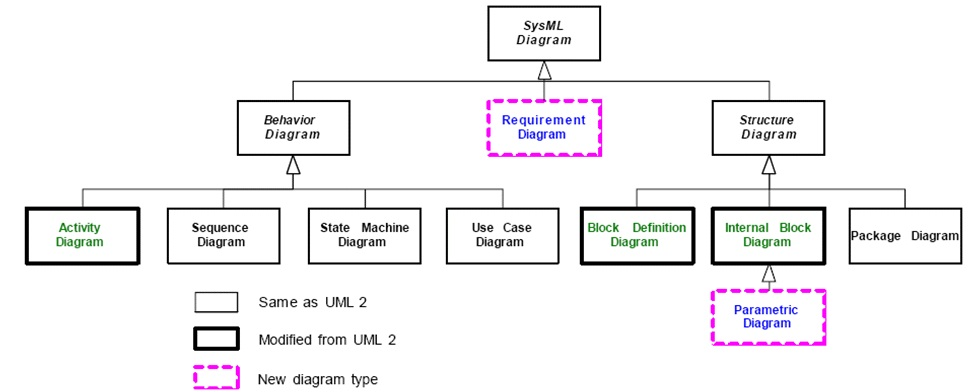
\includegraphics[scale=0.45]{./images/image5.jpg}

\end{frame}

%

\subsection{Automate d'interface}
\begin{frame}{}
    \centering
    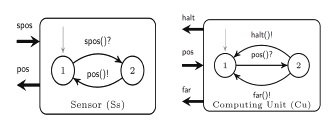
\includegraphics[scale=0.9]{./images/exempleAutomateInterface.jpg}
    \begin{block}{D�finition}
        \begin{itemize}
            \item Introduit par Alfaro et Henzinger
            \item Mod�lise les interface des composants
            \item Description des actions internes/entr�e/sortie

        \end{itemize}

    \end{block}

\end{frame}

%

\subsection{Vue globale du projet}
\begin{frame}{}
    \centering
    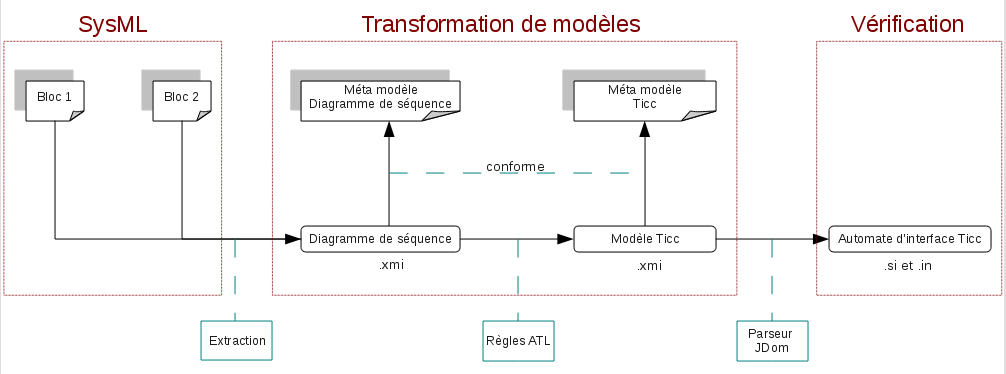
\includegraphics[scale=0.45]{./images/vueEnsemble.png}

\end{frame}





    \section{Outils utilis�s}

\subsection{Environnement de mod�lisation}
\begin{frame}{TopCased}
    \begin{block}{Pr�sentation}
        \begin{itemize}
            \item Analyse d'exigences
            \item Mod�lisation et simulation de mod�les
            \item G�n�ration de code
            \item Application RCP ou plugin Eclipse

        \end{itemize}

    \end{block}

\end{frame}

%

\subsection{R�gles de transformation}
\begin{frame}{ATL Transformation Language}
    \centering
    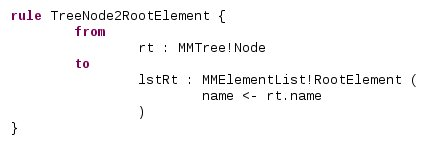
\includegraphics[scale=0.5]{./images/imageATL.jpeg}

    \begin{block}{Pr�sentation}
        \begin{itemize}
            \item Inclus avec TopCased
            \item Langage utilis� dans la transformation de mod�les
            \item Permet d'�crire les correspondances entre 2 �l�ments
            \item R�gles contenant du code OCL

        \end{itemize}

    \end{block}

\end{frame}

%

\subsection{V�rification de compatibilit�}
\begin{frame}{Tool for Interface Compatibility and Composition}
    \centering 
    \begin{columns}
        \begin{column}{0.4\linewidth}
            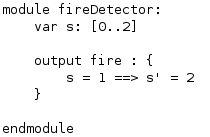
\includegraphics[scale=0.5]{./images/imageTiccParse.jpeg}

        \end{column}

        \begin{column}{0.3\linewidth}
            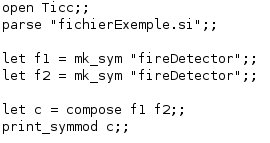
\includegraphics[scale=0.5]{./images/imageTiccExec.jpeg}

        \end{column}

    \end{columns}

    \begin{block}{Pr�sentation}
        \begin{itemize}
            \item Cr�� par notamment par Alfaro
            \item Permet de d�finir des automates d'interface et de les composer 
            \item Poss�de un langage qui lui est propre
            \item Formalise des composants
            \item Utilisation : Un fichier composant .si et un ex�cutable (OCaml) .in

        \end{itemize}

    \end{block}

\end{frame}



    \section{R�alisation}

\subsection{Transformation de mod�les}
\begin{frame}{M�ta mod�le}
	\begin{block}{Signification}
		\begin{itemize}
			\item Grec \textit{m�ta} : changement, succession, transformation
			\item Niveau d'abstraction sup�rieur
			\item Un mod�le repr�sentant un mod�le
		
		\end{itemize}			
	
	\end{block}

\end{frame}

\begin{frame}{Transformation de mod�les}
	\centering
	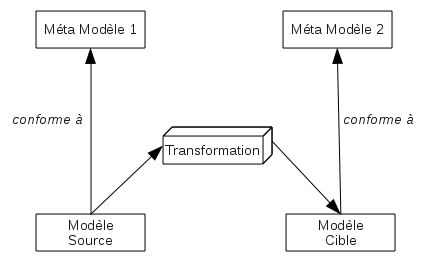
\includegraphics[scale=0.5]{./images/exogene.png}

	\begin{block}{Passage d'un mod�le � un autre}
		\begin{itemize}
			\item Mod�le source conforme � son m�ta mod�le
			\item Mod�le cible conforme � son m�ta mod�le
			\item Application de r�gles de transformation en utilisant les m�ta mod�les source et cible
		
		\end{itemize}			
	
	\end{block}

\end{frame}

%

\subsection{Les m�ta mod�les}
\begin{frame}{Diagramme de s�quences}
    \centering
    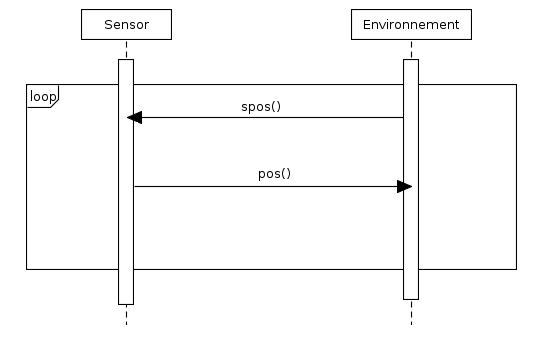
\includegraphics[scale=0.25]{./images/diagSeqExemple.png}

    \begin{block}{Simplifications}
        \begin{itemize}
            \item Red�finition de noms
            \item Abandon synchronisation des messages
            \item Garde les �l�ments utiles
            \item Ajoute de nouveaux �l�ments

        \end{itemize}

    \end{block}

\end{frame}

\begin{frame}{M�ta mod�le du diagramme de s�quences SysML}
    \centering
    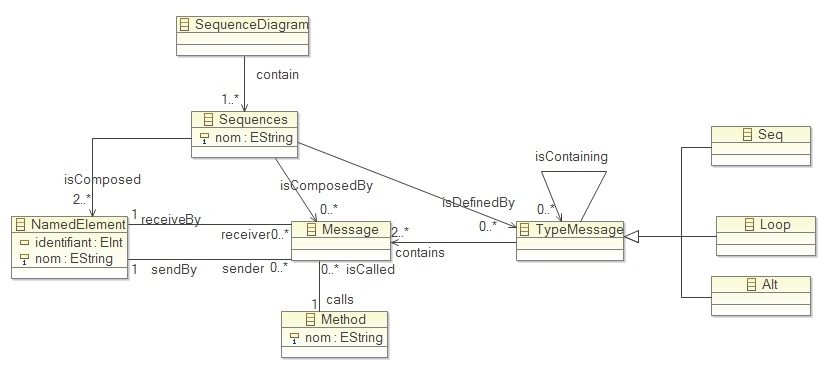
\includegraphics[scale=0.5]{./images/MMDiagSeq.jpg}

\end{frame}

\begin{frame}{M�ta mod�le du langage Ticc}
    \centering
    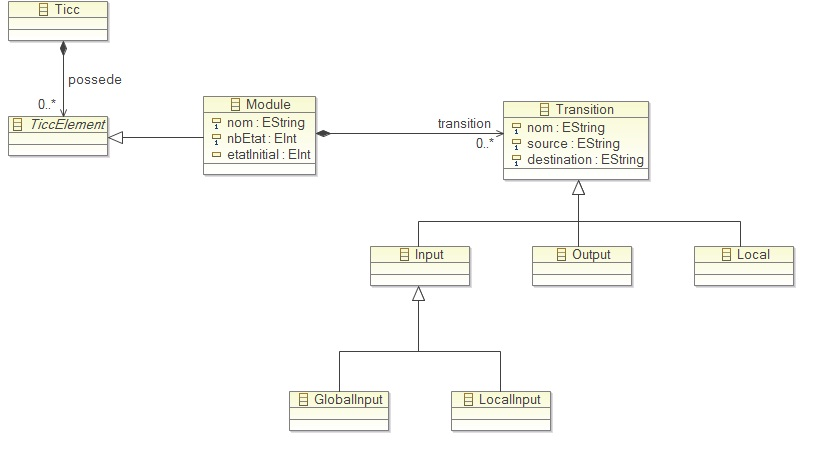
\includegraphics[scale=0.5]{./images/MMTicc.jpg}

\end{frame}

%

\subsection{Exemple fichier conforme au diagramme de s�quences}
\begin{frame}{\'Ecriture d'un fichier d'entr�e}
    \begin{block}{Explications}
        \begin{itemize}
            \item Fichier de type XMI (XML Metadata Interchange)
            \item Conforme au m�ta mod�le du diagramme de s�quences
            \item Contient deux s�quences
            \item Une s�quence re�oit/envoi des messages de/� l'ext�rieur 
            vers un composant appel� \textit{Environnement} 

        \end{itemize}

    \end{block}

\end{frame}

%

\subsection{R�gles ATL}
\begin{frame}{But des r�gles ATL}
    \centering
    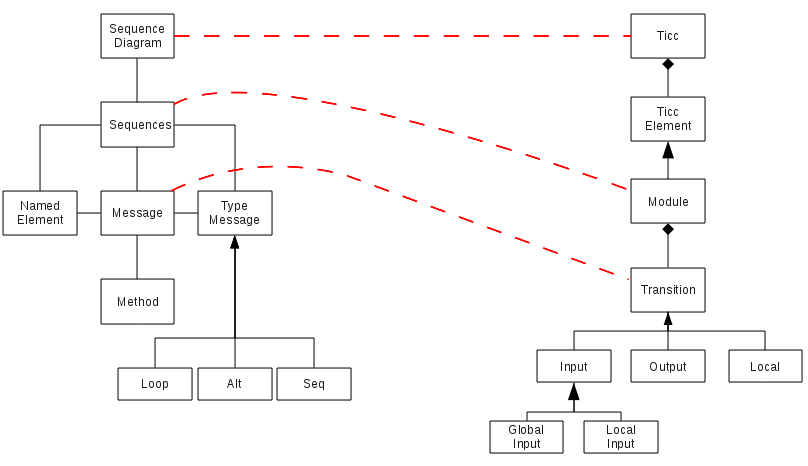
\includegraphics[scale=0.5]{./images/figureSimilitudeSeqTicc.png}

\end{frame}

%

\subsection{Parseur XML}
\begin{frame}{Parseur XML}
    \centering
    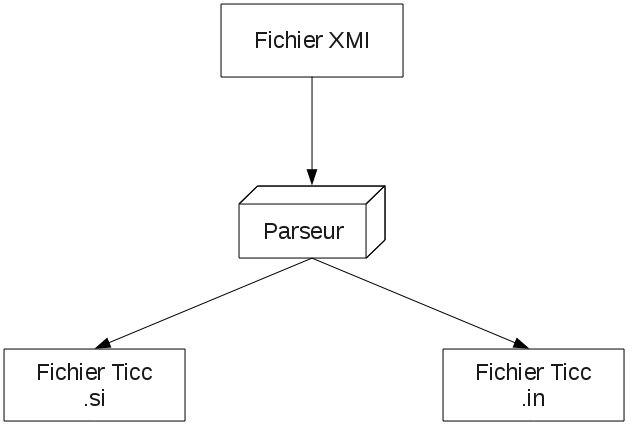
\includegraphics[scale=0.3]{./images/figureParseur.jpg}

    \begin{block}{Fonctionnement}
        \begin{itemize}
            \item Fichier de sortie XMI conforme Ticc 
            \item Traitement avec JDom
            \item G�n�ration fichier .si contenant les modules
            \item G�n�ration fichier .in ex�cutable OCaml

        \end{itemize}

    \end{block}

\end{frame}

%

\subsection{V�rification avec Ticc}
\begin{frame}{V�rification avec Ticc}
	\begin{block}{Principes}
		\begin{itemize}
			\item V�rification de compatibilit� de deux modules
			\item Utilisation des fichiers .si et .in
			\item Actuellement un fichier r�sultat trop volumineux
		
		\end{itemize}	
	
	\end{block}

\end{frame}



    \section{Bilan et Perspectives}
\begin{frame}{Bilan et perspectives}
	\begin{block}{Bilan}
		\begin{itemize}
			\item Transformation de mod�le 
			\item Ouverture � la v�rification de compatibilit�
		
		\end{itemize}
	
	\end{block}

	\begin{block}{Perspectives}
		\begin{itemize}
			\item Automatiser le processus avec un plugin Eclipse	
			\item Adapter un algorithme de parcours de BDD		
		
		\end{itemize}
	
	\end{block}

\end{frame}

\section*{}
\begin{frame}
	\centering
	\LARGE{Merci de votre attention.}

\end{frame}

\end{document}
